\documentclass[revtex4-2]{mpltx}
\usepackage{physics}

\begin{document}
\title{利用磁光克尔效应测定样品的磁滞回线}
\author{方尤乐}

\emailphone{eden@stu.pku.edu.cn}{(86)15313960363}
\affiliation{北京大学物理学院\quad 学号: 2000012416}
\begin{abstract}
    本实验通过观察不同外磁场下铁磁样品表面反射光的偏振变化,测得了样品的磁滞回线,来研究磁光克尔效应。
    实验利用光弹调制器和锁相放大器定量分析了磁光克尔效应的出射光,测量了不同磁场大小下的克尔转角和克尔椭偏率,
    由此获得了克尔磁滞回线,测得了样品的饱和克尔转角与矫顽力。
\end{abstract}
\keywords{磁光克尔效应,磁滞回线,克尔转角,克尔椭偏率}
\maketitle
\section{引言}
    1877 年,克尔(J. Kerr)发现平面偏振光从光洁磁极表面反射时,偏振面会发生微小偏转。这被称为磁光克尔效应,是一种探测物质磁化状态
    的光学方法。早在 20 世纪 50 年代,磁光克尔效应就被用于观察样品表面的磁畴结构,后来又以磁光克尔效应为基础发展出磁光存储技术。近年来,克尔效应被用于
    超薄磁性膜,磁化动态过程和自旋霍尔效应研究。作为一门将物质磁性和光偏振联系在一起的效应,磁光克尔效应在自旋电子学的科学研究和技术应用方面起着越来越
    重要的作用。本实验希望通过观察一个磁性介质对入射线偏振光的反射随外磁场的变化,测量克尔磁滞回线,来研究磁光克尔效应,并分析背后的物理机制。
\section{实验装置}
    实验装置如图\ref{fig:1}所示,入射激光经起偏器的线偏振光,近似垂直入射样品表面;
    出射光经光弹调制、检偏、光电探测转化为电信号,进而由锁相放大提取出谐波分量,
    输入计算机。外磁场同样由计算机控制,通过调整励磁电流以调整外磁场 B 的大小,
    利用高斯计监测并反馈调节所需磁场。
    \begin{figure}[htbp]
        \centering
        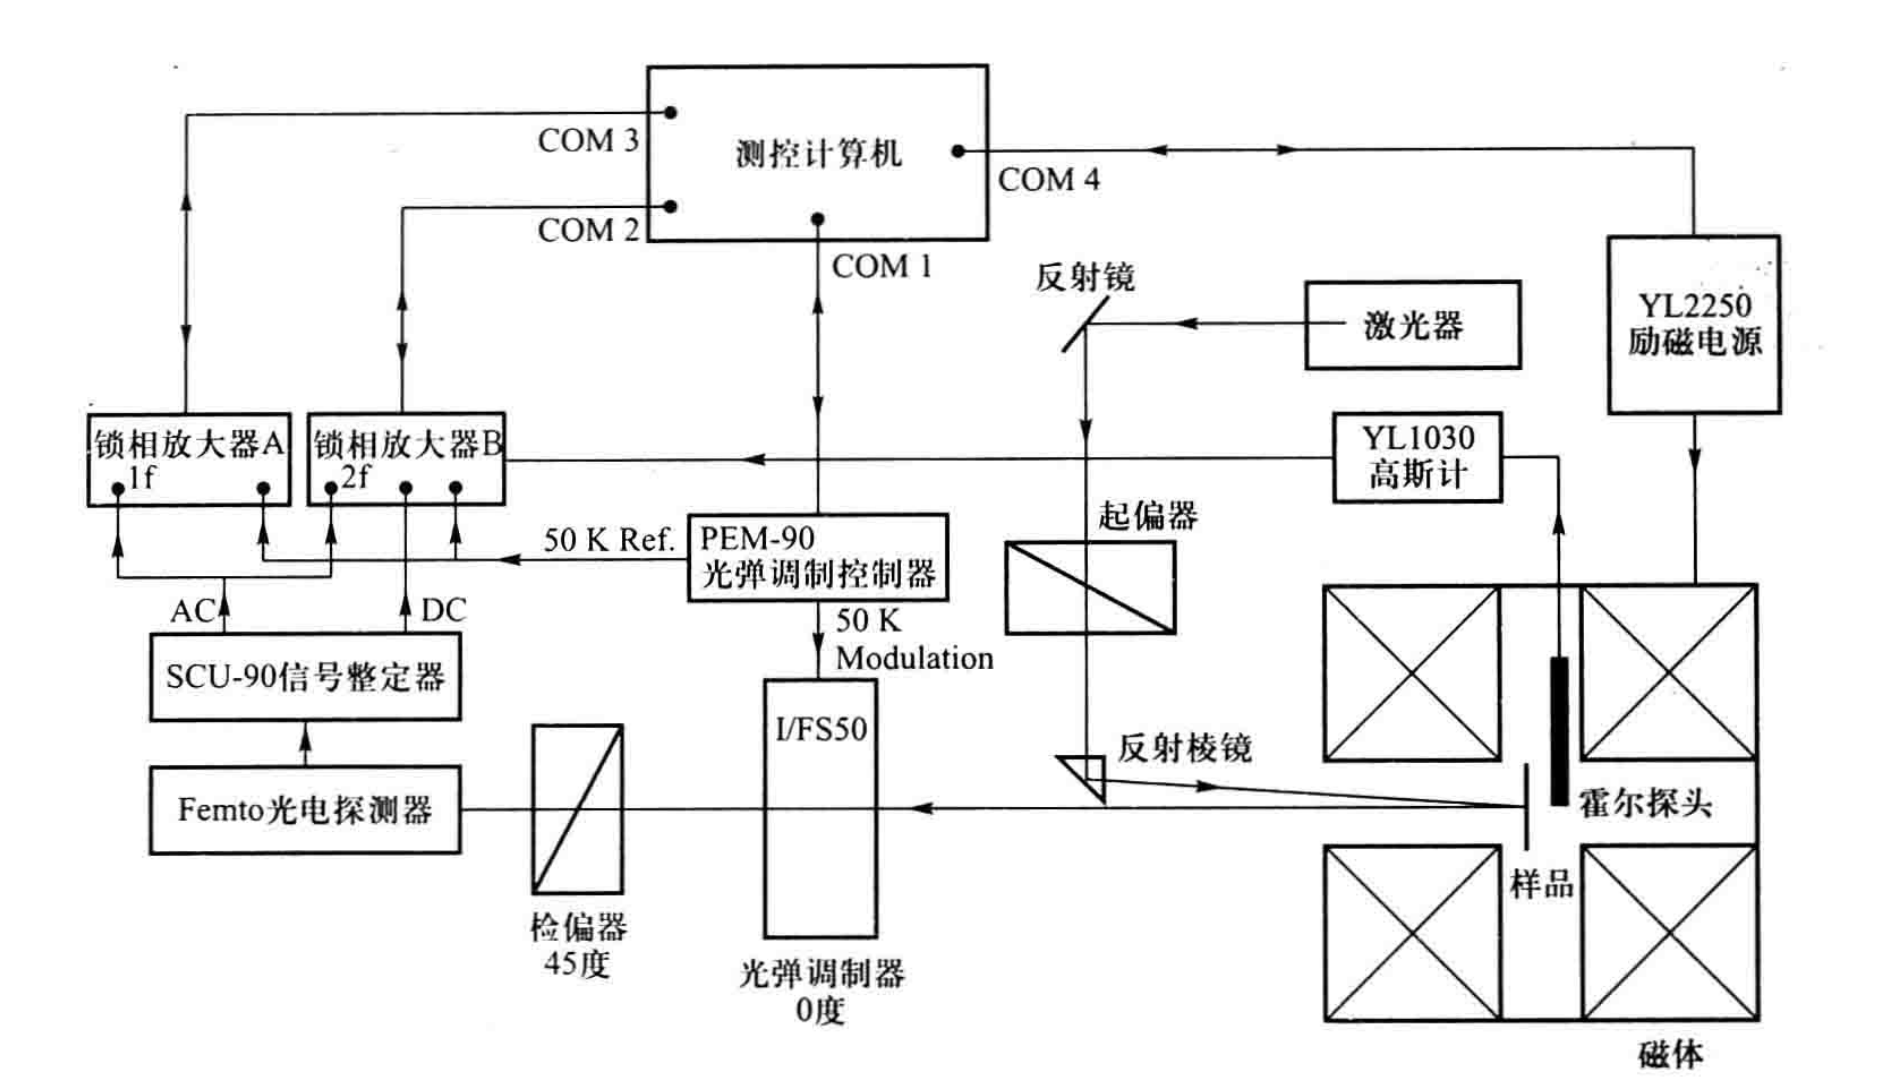
\includegraphics[width=0.8\textwidth]{./1.png}
        \caption{实验装置示意图}\label{fig:1}
    \end{figure}

    实验前首先调整好光路,通过观测反射光的光强调节样品表面的位置和朝向,使入射激光近似垂直入射样品表面。
    设入射偏振光的方向为 $y$ 方向,依次调节检偏器和光弹调制器,保证光弹调制器振动轴沿 $x$ 方向(与 $y$ 方向正交),
    检偏器方向与 $x$ 方向成 $45^\circ$,通过光弹调制器和检偏器实现对反射光偏振态的检测。
    调节光弹调制器的相位调制振幅为 $\delta_0=\delta_{J_0}=2.405$(零阶贝塞尔函数的零点),
    这样可以从锁相放大器提取出的直流分量、一次谐波分量和二次谐波分量直接地推出
    克尔转角和克尔椭偏率:
    \begin{align}
        \label{eq:1}&\theta_k = B\frac{V_{2\omega}}{4V_{0}J_2(\delta_{J_0})}\\
        \label{eq:2}&\varepsilon_k = B\frac{V_\omega}{4V_{0}J_1(\delta_{J_0})}
    \end{align}
    上式中系数 $B$ 未知,这是由于信号整定器额外引入了未知的放大系数,
    需要对它进行定标,这通过改变入射偏振方向 $0.5^\circ, 1^\circ, 1.5^\circ,\cdots, 2.5^\circ$,测定小角近似下 $\theta_k$ 的线性变化,
    通过最小二乘法给系数 $B$ 定标。
\section{结果与分析}
    首先通过计算机半自动地实现对 $B$ 的定标,由于小角度近似和调节入射偏振角度对应的起偏器角度时存在误差,
    通过最小二乘法得到的对 $B$ 的定标存在误差。

    测定 $\theta_0 = 0^\circ$ 时的克尔转角和克尔椭偏率,得到的结果如图\ref{fig:2}所示。
    
    \begin{figure}[htbp]
        \centering
        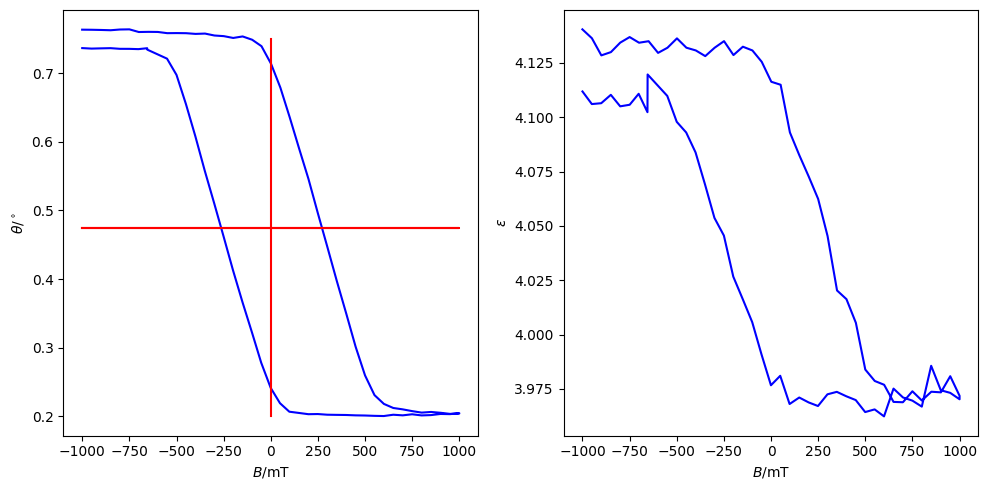
\includegraphics[width=0.8\textwidth]{./2.png}
        \caption{$\theta_0 = 0^\circ$ 时的克尔转角和克尔椭偏率}\label{fig:2}
    \end{figure}

    由图可以看到克尔转角的曲线体现了磁滞回线的特点:中心对称,存在饱和克尔转角。克尔转角曲线的左上角没有形成闭合的回路,
    可能是由于实验测定的过程中仪器收到了环境振动带来的干扰,导致起偏器角度或者光弹调制器角度漂移,导致测得的
    克尔转角曲线和克尔椭偏率曲线都没有闭合。克尔椭偏率的变化抖动幅度大,可能是因为光线在通过
    光弹调制晶体时发生反射和干涉,影响了第一谐波分量 $V_\omega$,从而影响了克尔椭偏率的测定。

    克尔转角曲线的 $\frac{\theta_{\max}+\theta_{\min}}{2}$ 没有位于 $\theta=0^\circ$ 的位置,
    这是由于在调整光路的时候,很难严格精确地控制起偏器偏振方向与光弹调制器振动方向正交。

    由于克尔转角曲线的误差较小,可以仍然用它来估计样品的饱和克尔转角和矫顽力。
    饱和克尔转角由 $\theta_{\text{饱和}}=(\theta_{\max}-\theta_{\min})/2$ 给出:
    \begin{align*}
        \theta_{\text{饱和}}=(\theta_{\max}-\theta_{\min})/2
        =0.475^\circ
    \end{align*}
    矫顽力由克尔磁滞回线与 $\theta=(\theta_{\max}+\theta_{\min})/2$ 的两个交点计算得到:
    \begin{align*}
        B_0=274.9\ \text{mT}
    \end{align*}

    依次调节起偏器至 $\theta=\theta_0\pm 1^\circ,\theta_0\pm 2^\circ$,分别测定不同入射偏振角度下的克尔磁滞回线。得到的结果如图所示:
    \begin{figure}[htbp]
        \centering
        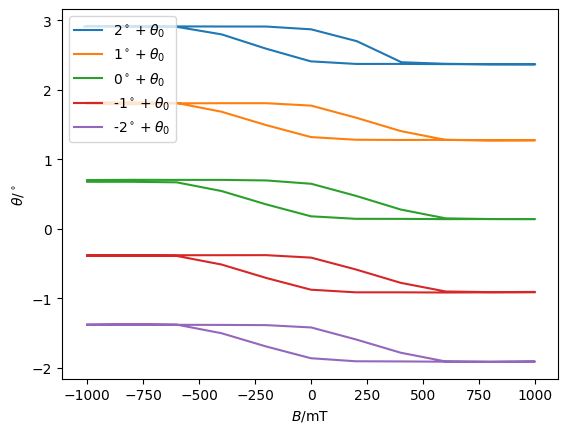
\includegraphics[width=0.8\textwidth]{./3.png}
        \caption{不同入射偏振角度下的克尔磁滞回线}\label{fig:3}
    \end{figure}
    
    可以看到克尔转角 $\theta$ 的位置随入射偏振角度的变化近似线性地平移,相邻两个克尔磁滞回线之间的距离近似为 $1^\circ$,
    这与起偏器变化的角度一致,所以符合理论预言。
    相邻两个克尔磁滞回线之间的距离不严格为 $1^\circ$,
    是因为小角度近似导致的误差,克尔转角与起偏器偏振角度不严格成线性关系,
    也是因为标定系数 $B$ 的误差。

\section{结论}
    本实验通过半自动化的现代手段,
    在不同外磁场下测定铁磁样品表面反射光的偏振变化,得到克尔转角和克尔椭偏率,
    从而测得了克尔磁滞回线,由此验证了磁光克尔效应。
    并进一步分析克尔磁滞回线,得到了样品的饱和克尔转角 $\theta_{\text{饱和}} \approx 0.475^\circ$ 
    及矫顽力 $B_0 \approx 274.9\ \text{mT}$。
\begin{acknowledgments}
    感谢周路群老师的细致指导,尤其是老师关于实验基本原理的启发对本人带来了
很大帮助;感谢合作者吴振翔同学的工作和帮助。
\end{acknowledgments}
\begin{thebibliography}{99}
    \bibitem{jindaishiyan} 吴思诚、荀坤. 近代实验物理[M]. 高等教育出版社, 2015.
\end{thebibliography}
\clearpage
\appendix
\section{思考题}
\subsection{我们的实验装置对克尔转角和克尔椭偏率的测量精度是否一样高,为什么?}
不一样高,从图 \ref{fig:2} 可以看到克尔椭偏率的测量精度是较低的,这可能是因为
光线在通过光弹调制器时发生反射和干涉,对一次谐波分量的影响较大,对二次谐波分量的影响较小,
所以根据式\eqref{eq:1}和式\eqref{eq:2},克尔椭偏率的测量精度较低。
\subsection{如果用一个以角速度 $\omega$ 旋转的 $\lambda/2$ 玻片代替光弹调制器,光电探测器的输出信号会如何变化,是否也能测出复克尔转角?}
$\lambda/2$ 波片会改变偏振光的方向,所以从样品表面反射的椭偏光经过
$\lambda/2$ 波片以后仍然是椭偏光,会以角速度 $2\omega$ 旋转。
那么无法从谐波分量中提取出克尔转角和克尔椭偏率的信息。
\end{document}